\documentclass{article}

\usepackage{arxiv}

\usepackage[utf8]{inputenc} % allow utf-8 input
\usepackage[T1]{fontenc}    % use 8-bit T1 fonts
\usepackage{lmodern}        % https://github.com/rstudio/rticles/issues/343
\usepackage{hyperref}       % hyperlinks
\usepackage{url}            % simple URL typesetting
\usepackage{booktabs}       % professional-quality tables
\usepackage{amsfonts}       % blackboard math symbols
\usepackage{nicefrac}       % compact symbols for 1/2, etc.
\usepackage{microtype}      % microtypography
\usepackage{graphicx}

\title{Assessing the influence of dopamine on the formation of
task-relevant visual routines}

\author{
    Kelly G. Garner
   \\
    School of Psychology \\
    University of New South Wales \\
  Sydney, NSW \\
  \texttt{\href{mailto:insert.unsw@here.edu.au}{\nolinkurl{insert.unsw@here.edu.au}}} \\
   \And
    Li-Ann Leow
   \\
    School of Psychology \\
    The University of Queensland \\
  St.~Lucia, QLD \\
  \texttt{} \\
   \And
    Aya Uchida
   \\
    School of Psychology \\
    The University of Queensland \\
  St.~Lucia, QLD \\
  \texttt{} \\
   \And
    Ole Jensen
   \\
    Center for Human Brain Health \\
    University of Birmingham \\
  Birmingham, UK \\
  \texttt{} \\
   \And
    Marta Garrido
   \\
    School of Psychological Sciences \\
    University of Melbourne \\
  Melbourne, VIC \\
  \texttt{} \\
   \And
    Paul E. Dux
   \\
    School of Psychology \\
    The University of Queensland \\
  St.~Lucia, QLD \\
  \texttt{} \\
  }


% tightlist command for lists without linebreak
\providecommand{\tightlist}{%
  \setlength{\itemsep}{0pt}\setlength{\parskip}{0pt}}

% From pandoc table feature
\usepackage{longtable,booktabs,array}
\usepackage{calc} % for calculating minipage widths
% Correct order of tables after \paragraph or \subparagraph
\usepackage{etoolbox}
\makeatletter
\patchcmd\longtable{\par}{\if@noskipsec\mbox{}\fi\par}{}{}
\makeatother
% Allow footnotes in longtable head/foot
\IfFileExists{footnotehyper.sty}{\usepackage{footnotehyper}}{\usepackage{footnote}}
\makesavenoteenv{longtable}

% Pandoc citation processing
\newlength{\cslhangindent}
\setlength{\cslhangindent}{1.5em}
\newlength{\csllabelwidth}
\setlength{\csllabelwidth}{3em}
\newlength{\cslentryspacingunit} % times entry-spacing
\setlength{\cslentryspacingunit}{\parskip}
% for Pandoc 2.8 to 2.10.1
\newenvironment{cslreferences}%
  {}%
  {\par}
% For Pandoc 2.11+
\newenvironment{CSLReferences}[2] % #1 hanging-ident, #2 entry spacing
 {% don't indent paragraphs
  \setlength{\parindent}{0pt}
  % turn on hanging indent if param 1 is 1
  \ifodd #1
  \let\oldpar\par
  \def\par{\hangindent=\cslhangindent\oldpar}
  \fi
  % set entry spacing
  \setlength{\parskip}{#2\cslentryspacingunit}
 }%
 {}
\usepackage{calc}
\newcommand{\CSLBlock}[1]{#1\hfill\break}
\newcommand{\CSLLeftMargin}[1]{\parbox[t]{\csllabelwidth}{#1}}
\newcommand{\CSLRightInline}[1]{\parbox[t]{\linewidth - \csllabelwidth}{#1}\break}
\newcommand{\CSLIndent}[1]{\hspace{\cslhangindent}#1}

\begin{document}
\maketitle


\begin{abstract}
Enter the text of your abstract here.
\end{abstract}

\keywords{
    blah
   \and
    blee
   \and
    bloo
   \and
    these are optional and can be removed
  }

\begin{verbatim}
## Loading required package: Rcpp
\end{verbatim}

\begin{verbatim}
## Loading 'brms' package (version 2.18.0). Useful instructions
## can be found by typing help('brms'). A more detailed introduction
## to the package is available through vignette('brms_overview').
\end{verbatim}

\begin{verbatim}
## 
## Attaching package: 'brms'
\end{verbatim}

\begin{verbatim}
## The following object is masked from 'package:stats':
## 
##     ar
\end{verbatim}

\hypertarget{introduction}{%
\section{Introduction}\label{introduction}}

Here goes an introduction text

\hypertarget{methods}{%
\section{Methods}\label{methods}}

\label{sec:Methods}

\hypertarget{participants}{%
\subsection{Participants}\label{participants}}

A total of 40 participants (mean age: 24.5, sd: 5, 30 female, 10 male)
were recruited using the undergraduate and paid SONA pools administered
by the University of Queensland. All procedures were cleared by the
University of Queensland Human Research ethics committee
{[}2017/HE000847{]}, and were conducted in accordance with the National
Statement on Ethical Conduct in Human Research. Participants were over
18 years old, had no known neurological and psychiatric conditions
(assessed by self report), and no contraindications to Levodopa, as
assessed by the Levodopa safety screening questionnaire. Informed
consent was obtained at the start of the first session.

\hypertarget{procedure}{%
\subsection{Procedure}\label{procedure}}

Participants attended two sessions, spaced approximately 1 week apart.
After initial blood pressure and mood assessments, participants received
either placebo (vitamin C) or Levodopa (Madopar 125: 100 mg Levodopa and
25 mg Benserazide Hydrochloride), crushed and dispersed in orange juice,
now referred to as the `placebo' and `DA' sessions respectively. The
solution was prepared by an experimenter who did not administer the
remaining experimental procedures. This protocol was sufficient to
achieve double blinding in previous work
(\textbf{chowdhuryDopamineModulatesEpisodic2012?};
\textbf{chowdhuryDopamineRestoresReward2013?}). Participants then
completed the Five Facet Mindfulness Questionnaire
(\textbf{baerUsingSelfReportAssessment2006?}) and the Barratt
Impulsivity Scale {[}BIS;
(\textbf{pattonFactorStructureBarratt1995?}){]}, as trait impulsivity
scores are associated with midbrain dopamine D2/D3 receptor
availability. Around 30 minutes after drug administration, participants
completed a second blood pressure and mood rating assessment.
Participants then completed the practice stage of the task, so that the
experimental stage began approximately 40 minutes after drug ingestion,
within the window of peak plasma availability. At the end of the
session, participants completed the final blood pressure and mood rating
assessment and were asked whether they thought they had been given the
active or placebo drug.

\hypertarget{apparatus}{%
\subsection{Apparatus}\label{apparatus}}

The experimental task was run with custom code\footnote{\url{https://github.com/kel-github/variability-decision-making}},
written using Matlab 2012b (32 bit) and Psychtoolbox v3.0.14, on a
Windows 7 (64-bit) on a Dell Precision T1700 desktop computer, displayed
using a ASUS VG248 monitor. Gaze coordinates (x, y) were sampled at 120
Hz using a monitor-mounted iView Red-m infrared eye tracker
(SensoMotoric Instruments GmbH, Teltow, Germany). Participants were
seated from the monitor at an approximate viewing distance of 57 cm, and
positioned on a chin-rest for the duration of the task.

\hypertarget{experimental-task}{%
\subsection{Experimental Task}\label{experimental-task}}

Each trial began with a fixation dot presented centrally on a grey
screen {[}RGB: 200 200 200{]}. Participants were instructed to fixate on
the dot to begin a trial. After 1000 ms of continuous correct fixation
samples (within 100 pixels of fixation), a square was presented that
comprsed 18° of degree visual angle along each length. The square could
be one of four possible colours {[}RGBs: 87, 208, 169; 267, 145, 52;
167, 162, 229; 239, 91, 158{]}. After 1000 ms, a 4 x 4 grid of smaller
squares appeared within the larger square, in a darker version of the
background colour ({[}RGB{]}-50). Each square comprised 2.6° of visual
angle. Participants were instructed that the 4 x 4 grid represented
doors, and that they were to use their eyes to open the doors to find
where the target was hiding. Participants were also instructed that they
were to fixate on a single door to open it. When participants had
fixated on a single door for over 300 ms, the door either turned black
{[}RGB: 50, 50, 50{]}, to denote the absence of a target, or the target
was displayed and the trial was terminated. If the door had turned
black, it returned to its previous colour as soon as it was detected
that the participant had moved their eyes from the door. Targets were
animal images drawn randomly on each trial from a pool of 100 images
taken from the internet. The time at which the target was available to
be found varied from trial to trial, with the onset being drawn from a
uniform distribution between 500-2000 ms. Once the target was available
and the correct door selected, the target was displayed for 750 ms. Upon
termination of the trial, the grey screen and white fixation cross were
presented (Fig @ref(fig:taskFig)A).

In each session, participants were shown two possible background and
door colour sets. Participants were instructed that each colour
represented a world, and that the animals had different places they
preferred to hide, depending on the world they were in. There were four
possible target locations within each world, or from here on, visual
context. For each visual context, 1 door from each quadrant was selected
as one of the 4 target locations where the targets could appear (see Fig
@ref(fig:taskFig)B), with the constraint that target locations could not
overlap between contexts. Thus each colour reflected a context in which
participants could establish a set of task-relevant eye-movements,
i.e.~towards the 4 possible target locations for that context. Note that
within each context, the target was equally likely to appear behind any
one of the 4 target doors (p=.25) and would never appear behind the
remaining doors (p=0). Colour-target location mappings were
counterbalanced across participants, as was the assignment of coloured
contexts to sessions. Participants completed 80 trials in each context.
Eye-movement calibration and validation was performed every 20 trials.
Participants were also shown the standard QWERTY keyboard and were
instructed that they could press `x' at any time to perform a new
calibration and validation if they felt that their eye-movements were no
longer being registered accurately; i.e.~if they were unable to open
doors even though they were selecting them.

\begin{figure}

{\centering 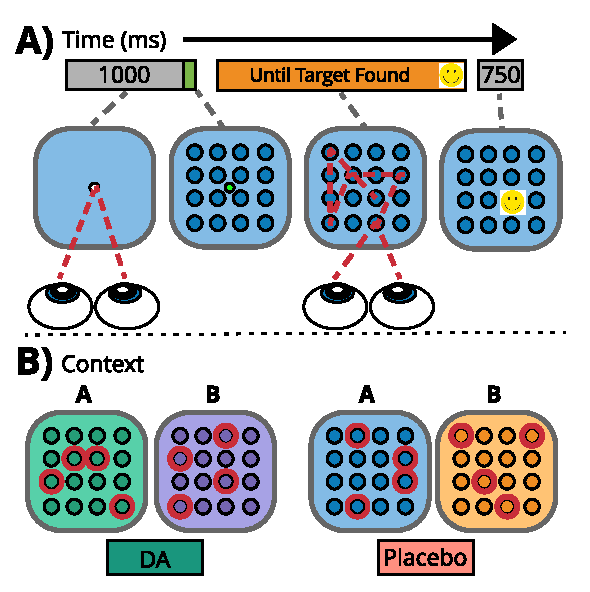
\includegraphics[width=0.7\linewidth]{../../images/DA_ExpTask} 

}

\caption{Experimental Task. A) A single trial where participants use their eyes to open doors to locate a target. B) Contexts and sessions: in each session, participants are exposed to two colour contexts each with 4 unique and equiprobable target locations. Colours and target locations were counterbalanced across participants and sessions. In each session, Levodopa (DA) or placebo is administered under double blind conditions.}\label{fig:taskfig}
\end{figure}

\hypertarget{statistical-approach}{%
\subsection{Statistical Approach}\label{statistical-approach}}

The analysis was designed to assess the learning of the target locations
given the context, the extent to which eye-movements became
stereotypical, and how both of these measures were modulated by the
dopamine and mindfulness factors. All custom analysis code is available
online\footnote{insert link}. The analysis was performed using R and
RStudio v2022.07.2 (\textbf{rstudiocitation?}), and can be reproduced in
the Neurodesk container environment
(\textbf{rentonNeurodeskAccessibleFlexible2022?}).

\hypertarget{data-cleaning}{%
\subsubsection{Data cleaning}\label{data-cleaning}}

Doors were marked as selected if participants gazed at them for a
duration of at least 300 ms. We assumed that a door could not be
selected twice consecutively, and collapsed any consecutive selections
into a single door selection. Last, as the final door selection of every
trial was fixed (i.e.~finding the target location ends the trial), we
removed the final selection from each trial for the sequence analysis
defined below. We excluded data from one participant whose total number
of door selections was greater than 3 standard deviations from the mean
across both sessions. The remaining 39 datasets were retained for all of
the analyses. Note that this is more inclusive than our pre-registered
plan for data exclusions\footnote{\url{https://osf.io/2y6pk}}. Based on
pilot data, we had planned to exclude participants who scored
\textless{} 65\% accuracy over the course of a session. Analysis of the
final sample suggested that this was too stringent, as this resulted in
the exclusion of 14 of 40 participants.

\hypertarget{accuracy}{%
\subsection{Accuracy}\label{accuracy}}

We sought to determine the extent to which participants learned the
target locations, and whether participants learned to select the doors
that were relevant given the current context. Door selections were
classified as target relevant (TR) for the current context (cc), the
other context from that session (oc), or neither (n). Data was then
grouped into blocks of 10 trials per context, and grouped across
contexts, resulting in 8 blocks of 20 trials. First, to determine
whether participants learned the target locations, regardless of
context, we computed accuracy as the number of correct door selections
(referred to from now as accuracy {[}acc{]}), relative to all door
selections:

\[
acc = \frac{\sum{(TR_{cc}, TR_{oc})}}{\sum{(TR_{cc}, TR_{oc}, n)}}
\]

We assessed the influence of block, drug and mindfulness on accuracy
using a Bayesian mixed model approach. Accuracy was assumed to be drawn
from a binomial distribution (1=target door, 0 = non-target door), and
the probability of drawing a hit from the total number of door
selections made by a given participant was modelled using a logistic
regression, using default weakly informative priors on the regression
coefficients that are defined below. Note that as we use logistic
regression, resulting regression parameter values reflect changes to the
log-odds of correct door selections.

For this and following analyses, we sought to identified the model that
best fit the data, and then made inference over the resulting
parameters. We report the 95\% confidence intervals (CIs) of the
parameter posteriors, and assume we have detetected a reliable effect of
a parameter when the 95\% CIs of the posterior do not include zero.
Models were fit using the BRMS
(\textbf{burknerBrmsPackageBayesian2017?}) interface for Stan
(\textbf{standevelopmentteamStanModelingLanguage?}) and RStan
(\textbf{standevelopmentteamRStanInterfaceStan2023?}). We used the
default weakly informative priors as specified in
(\textbf{burknerBrmsPackageBayesian2017?}). Specifically, fixed and
random effect \(\beta\) coefficients were given a flat prior, intercept
and standard deviations were assumed to be drawn from a student's \(t\)
distribution (df=1, location=0, scale=2.5), and the LKJ-correlation
prior with parameter \(\zeta\) \textgreater{} 0 was used for the
parameter covariance matrix. For each model, we checked for parameter
recovery using simulated data. Furthermore, once fitted, we checked that
the residuals showed no signs of systematic error, that the chains had
converged, and that \(\hat{R}\) values were less than 1.01.

To eschew an overly large model space, and in line with our
pre-registration, we first fit models that containing each combination
of the block and drug regressors (and associated random effects), and
found the best model using leave-one-out (LOO) cross validation (as
implemented in \textbf{vehtariPracticalBayesianModel2017?}). (Note that
in the pre-registration document we had proposed to compare models using
the deviance information criterion (DIC). As LOO is more robust than DIC
to influential observations, and is readily implemented for use with
BRMS model objects, we opted to use LOO instead of DIC). Upon
identifying the best model from the experimentally manipulated
regressors, we then added the mindfulness regressor in all possible
combinations with the best model for the experimental effects, and once
again selected the best model (as evidenced by LOO). Last we controlled
for trait impulsivity by adding BIS scores as a main effect to the
winning model. Note that in no cases did adding BIS scores improve the
model, as assessed by LOO. We report the difference in the expected log
posterior density (ELPD) between the winning model and the next best
models, and the ratio of the ELPD difference to the standard error (SE)
of the difference (ELPD:SE). The full set of model comparisons are
presented in the supplementary materials. Note that this value suggests
the difference between the model ELPD's in units of SE.

\hypertarget{contextual-accuracy}{%
\subsection{Contextual Accuracy}\label{contextual-accuracy}}

We also sought to understand whether dopamine modulates the ability of
participants to select the correct door, given the context. Therefore,
for each context, we computed the total number of cc door selections
(c-acc), and modelled the probability of attaining c-acc given the total
number of correct door selections:

\[
c-acc = \frac{\sum{TR_{cc}}}{\sum{(TR_{cc}, TR_{oc})}}
\]

We then fit this data with Bayesian mixed effects models following the
procedure above (Note that in the pre-registration document we had
suggested to include a regressor for context. Visual inspection of the
data showed that c-acc was highly comparable across contexts {[}see
supplemental figures{]}. We therefore opted to simplify the model space
and collapse over this factor).

\hypertarget{stereotypical-sequences}{%
\subsection{Stereotypical sequences}\label{stereotypical-sequences}}

Next, we seek to determine the extent to which door-selection patterns
become more stereotypical over the course of the task, and whether
dopamine and mindfulness modulates the extent of stereotypy. Here we
define stereotypy as sets of door selections being deployed in the same
order, over trials. Therefore we wish to know whether, given the set of
doors that a participant chose to open over the trials of the
experiment, does their data suggest that they are selecting them in a
more regularised manner as the experiment progresses?

In order to characterise the extent to which door selections increased
in stereotypicality, we reasoned that participants showing more
stereotypical door selections should show an increase in a given subset
of transition probabilities, and a decrease in lesser or unused door
transitions. This stands in contrast to someone who is making door
selections in an exploratory, or non-stereotyped way, where a greater
set of door transition probabilities should show higher probability.
Therefore, the transition matrices of individuals engaged in
stereotypical door selections should show higher variance than those who
are not engaging in stereotypical door selections. We therefore omputed
transition probability matrices for each participant, session, block and
context, and computed the variance of each matrix. Variances were then
collapsed across context to form a single variance score for each
participant, session and block.

The resulting variance scores were subject to a comparable Bayesian
mixture modelling approach as is described for the accuracy data above
with a few key differences; the variance scores were assumed to be drawn
from a skewed normal distribution whose mean was defined by the
regression parameters. \(\sigma\) was assumed to be drawn from a
Student's t distribution (df=3, location=0, scale=2.5), the skew
parameter was assumed to be drawn from a normal distribution
\(\mathcal{N}(0,4)\). The remaining priors for the intercept,
beta-coefficients and covariances were defined in the same manner as for
the accuracy data models. As the log-log plot of V vs block suggested a
power function, analysis was performed on the logged data so that the
relationship between the regressors and the computed V values was best
described by a straight line. Identification of the winning model
proceeded as described for the accuracy data above.

\hypertarget{blinding-analyses}{%
\subsection{Blinding analyses}\label{blinding-analyses}}

To determine whether awareness of the dopamine intervention could have
contributed to the findings, the probability of participant and
experimenter ratings were compared to the expected values assuming
chance guessing, using a binomial model. Blood-pressure and mood
measures were compared using {[}insert whether paired t-test or
Mann-Whitney U test{]}.

\hypertarget{results}{%
\section{Results}\label{results}}

HERE I INSERT THE BRIEFEST OVER VIEW OF ALL THE RESULTS

\hypertarget{accuracy-1}{%
\subsection{Accuracy}\label{accuracy-1}}

\hypertarget{model-selection}{%
\subsubsection{Model Selection}\label{model-selection}}

For the accuracy data, the winning model contained main effects of
block, drug, mindfulness, as well as a block x mindfulness, a drug x
mindfulness and a block x drug x mindfulness interaction. This model was
very closely preferred to the next best model, which was the same except
for the 3-way interaction (ELPD diff = -0.01, ELPD:SE = -0.01). However,
this model was more strongly preferred than those containing no
interactions between mindfulness and the block and drug factors (ELPD
diff = -11.94, ELPD:SE = -1.87), and the one that did not include an
effect of mindfulness (ELPD diff = -12.02, ELPD:SE = -1.88). Adding the
BIS scores did not improve the predictive value of the model (ELPD diff
= -0.16, ELPD:SE = -0.34). Note that although we draw inferences over
parameters from the winning model, our inferences are the same as if we
had used the more complex model that includes the BIS scores, or the
next best model.

\hypertarget{the-effect-of-drug-and-mindfulness-on-acc}{%
\subsubsection{The effect of drug and mindfulness on
acc}\label{the-effect-of-drug-and-mindfulness-on-acc}}

Accuracy data are plotted by block and drug session (DA va placebo) are
shown in Fig Fig @ref(fig:accFig)A. In line with the notion that
dopamine and mindfulness may interact to support the learning of
appropriate sets of door selections, the winning model showed a drug x
mindfulness interaction that differed from zero (mean log odds = -0.11,
95\% CI{[}-0.16, -0.06{]}, Fig @ref(fig:accFig)E). To better understand
this interaction, we first computed a score for each participant that
reflected the overall change of accuracy due to levodopa administration.
To achieve this, we computed the average accuracy for each participant
and session, as predicted by the model, and took the difference between
the DA and placebo sessions (acc{[}DA - P{]}). Note that a positive
score indicates that performance was better in the DA session. Next we
examined the relationship between these scores and mindfulness scores.
As can be seen in Fig @ref(fig:accFig)B, there was a positive
relationship between the effect of DA and mindfulness; participants
scoring higher for mindfulness showed higher accuracy for the DA
relative to the placebo session, individuals scoring low on mindfulness
showed poorer accuracy on the DA relative to the placebo session. Thus
the impact of DA on the establishment of task-relevant eye-movement
sequences is dependent on the mindfulness state of the individual.

As can be seen from Fig @ref(fig:accFig)C, accuracy increased over
blocks (mean log odds = 0.15, 95\% CI{[}0.09, 0.22, Fig
@ref(fig:accFig)D). We also note that there was the suggestion of a main
effect of the drug intervention (mean log odds = 0.04, 95\% CI{[}-0.00,
0.09, Fig XX), however, the strength of this effect is presumably
modulated by the drug x mindfulness interaction.

\begin{figure}

{\centering 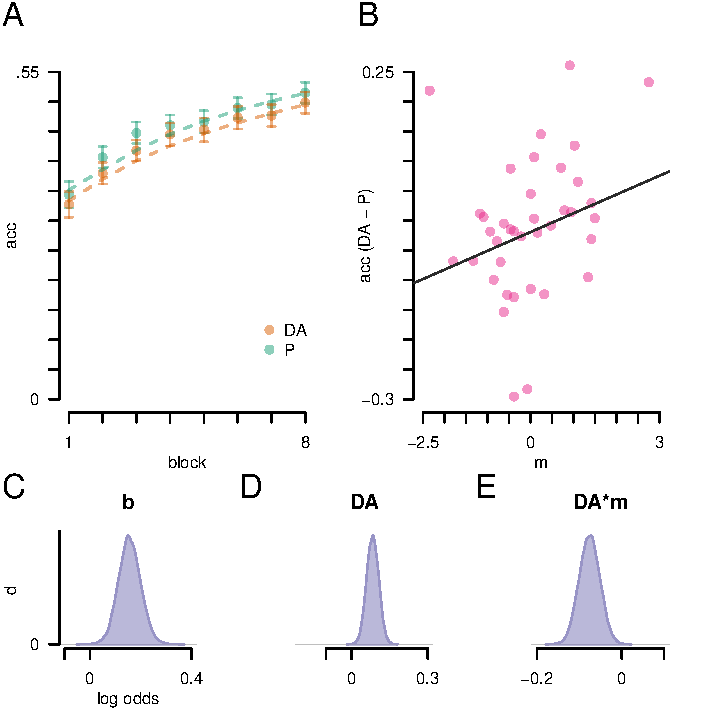
\includegraphics[width=0.7\linewidth]{../../images/acc_fig} 

}

\caption{The influence of dopamine and mindfulness on accuracy. A) Accuracy (acc) data by block and drug. Circles reflect observed average accuracy, dotted lines reflect the fit of the winning model. B) The association between trait mindfulness (x-axis) and the impact of drug on accuracy [DA-P]. The bottom row shows posterior densities (in log odds) estimated for C) the main effect of block (b), D) the main effect of DA, and E) the drug x mindfulness (m) interaction. DA = dopamine, P = placebo. Error bars reflect within-subject standard error of the mean [SE].}\label{fig:accfig}
\end{figure}

\hypertarget{contextual-accuracy-acc}{%
\subsection{Contextual accuracy (acc)}\label{contextual-accuracy-acc}}

\hypertarget{stereotypy}{%
\subsection{Stereotypy}\label{stereotypy}}

LaTeX command can be used to reference other section. See Section
\ref{sec:headings}. However, you can also use \textbf{bookdown}
extensions mechanism for this.

\hypertarget{headings-second-level}{%
\subsection{Headings: second level}\label{headings-second-level}}

You can use equation in blocks

\[
\xi _{ij}(t)=P(x_{t}=i,x_{t+1}=j|y,v,w;\theta)= {\frac {\alpha _{i}(t)a^{w_t}_{ij}\beta _{j}(t+1)b^{v_{t+1}}_{j}(y_{t+1})}{\sum _{i=1}^{N} \sum _{j=1}^{N} \alpha _{i}(t)a^{w_t}_{ij}\beta _{j}(t+1)b^{v_{t+1}}_{j}(y_{t+1})}}
\]

But also inline i.e \(z=x+y\)

\hypertarget{headings-third-level}{%
\subsubsection{Headings: third level}\label{headings-third-level}}

Another paragraph.

\hypertarget{examples-of-citations-figures-tables-references}{%
\section{Examples of citations, figures, tables,
references}\label{examples-of-citations-figures-tables-references}}

\label{sec:others}

You can insert references. Here is some text (Kour and Saabne 2014b,
2014a) and see Hadash et al. (2018).

The documentation for \verb+natbib+ may be found at

You can use custom blocks with LaTeX support from \textbf{rmarkdown} to
create environment.

\begin{center}
\url{http://mirrors.ctan.org/macros/latex/contrib/natbib/natnotes.pdf\%7D}

\end{center}

Of note is the command \verb+\citet+, which produces citations
appropriate for use in inline text.

You can insert LaTeX environment directly too.

\begin{verbatim}
   \citet{hasselmo} investigated\dots
\end{verbatim}

produces

\begin{quote}
  Hasselmo, et al.\ (1995) investigated\dots
\end{quote}

\begin{center}
  \url{https://www.ctan.org/pkg/booktabs}
\end{center}

\hypertarget{figures}{%
\subsection{Figures}\label{figures}}

You can insert figure using LaTeX directly.

See Figure \ref{fig:fig1}. Here is how you add footnotes. {[}\^{}Sample
of the first footnote.{]}

\begin{figure}
  \centering
  \fbox{\rule[-.5cm]{4cm}{4cm} \rule[-.5cm]{4cm}{0cm}}
  \caption{Sample figure caption.}
  \label{fig:fig1}
\end{figure}

But you can also do that using R.

\begin{figure}

{\centering 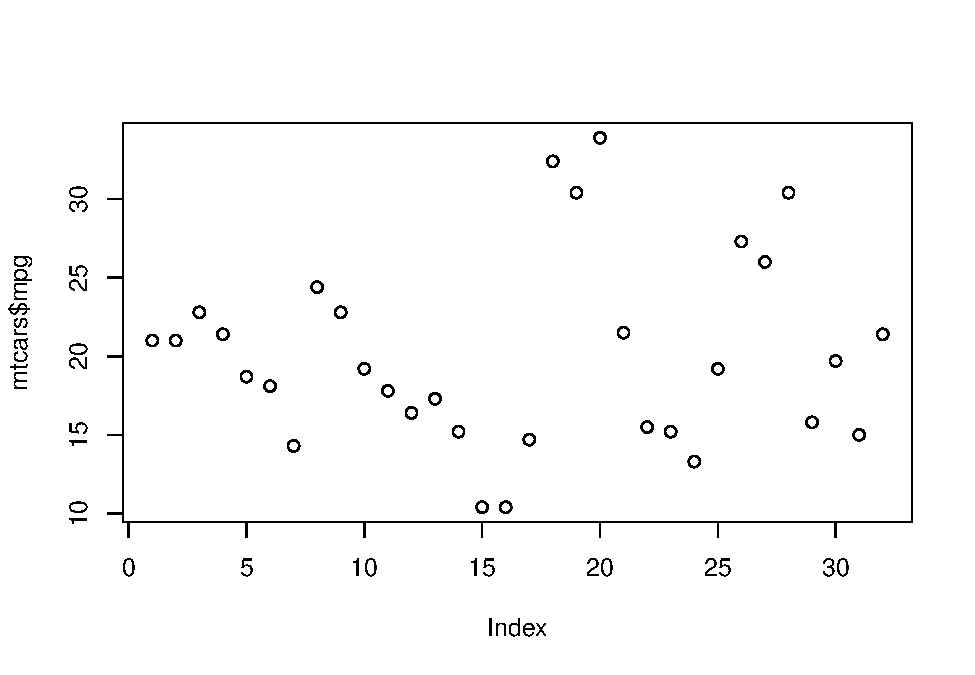
\includegraphics{assessing-the-role-of-dopamine-on-the-formation-of-contextually-relevant-visual-routines_files/figure-latex/fig2-1} 

}

\caption{Another sample figure}\label{fig:fig2}
\end{figure}

You can use \textbf{bookdown} to allow references for Tables and
Figures.

\hypertarget{tables}{%
\subsection{Tables}\label{tables}}

Below we can see how to use tables.

See awesome Table\textasciitilde{}\ref{tab:table} which is written
directly in LaTeX in source Rmd file.

\begin{table}
 \caption{Sample table title}
  \centering
  \begin{tabular}{lll}
    \toprule
    \multicolumn{2}{c}{Part}                   \\
    \cmidrule(r){1-2}
    Name     & Description     & Size ($\mu$m) \\
    \midrule
    Dendrite & Input terminal  & $\sim$100     \\
    Axon     & Output terminal & $\sim$10      \\
    Soma     & Cell body       & up to $10^6$  \\
    \bottomrule
  \end{tabular}
  \label{tab:table}
\end{table}

You can also use R code for that.

\begin{longtable}[]{@{}
  >{\raggedright\arraybackslash}p{(\columnwidth - 22\tabcolsep) * \real{0.2687}}
  >{\raggedleft\arraybackslash}p{(\columnwidth - 22\tabcolsep) * \real{0.0746}}
  >{\raggedleft\arraybackslash}p{(\columnwidth - 22\tabcolsep) * \real{0.0597}}
  >{\raggedleft\arraybackslash}p{(\columnwidth - 22\tabcolsep) * \real{0.0746}}
  >{\raggedleft\arraybackslash}p{(\columnwidth - 22\tabcolsep) * \real{0.0597}}
  >{\raggedleft\arraybackslash}p{(\columnwidth - 22\tabcolsep) * \real{0.0746}}
  >{\raggedleft\arraybackslash}p{(\columnwidth - 22\tabcolsep) * \real{0.0746}}
  >{\raggedleft\arraybackslash}p{(\columnwidth - 22\tabcolsep) * \real{0.0746}}
  >{\raggedleft\arraybackslash}p{(\columnwidth - 22\tabcolsep) * \real{0.0448}}
  >{\raggedleft\arraybackslash}p{(\columnwidth - 22\tabcolsep) * \real{0.0448}}
  >{\raggedleft\arraybackslash}p{(\columnwidth - 22\tabcolsep) * \real{0.0746}}
  >{\raggedleft\arraybackslash}p{(\columnwidth - 22\tabcolsep) * \real{0.0746}}@{}}
\caption{Head of mtcars table}\tabularnewline
\toprule()
\begin{minipage}[b]{\linewidth}\raggedright
\end{minipage} & \begin{minipage}[b]{\linewidth}\raggedleft
mpg
\end{minipage} & \begin{minipage}[b]{\linewidth}\raggedleft
cyl
\end{minipage} & \begin{minipage}[b]{\linewidth}\raggedleft
disp
\end{minipage} & \begin{minipage}[b]{\linewidth}\raggedleft
hp
\end{minipage} & \begin{minipage}[b]{\linewidth}\raggedleft
drat
\end{minipage} & \begin{minipage}[b]{\linewidth}\raggedleft
wt
\end{minipage} & \begin{minipage}[b]{\linewidth}\raggedleft
qsec
\end{minipage} & \begin{minipage}[b]{\linewidth}\raggedleft
vs
\end{minipage} & \begin{minipage}[b]{\linewidth}\raggedleft
am
\end{minipage} & \begin{minipage}[b]{\linewidth}\raggedleft
gear
\end{minipage} & \begin{minipage}[b]{\linewidth}\raggedleft
carb
\end{minipage} \\
\midrule()
\endfirsthead
\toprule()
\begin{minipage}[b]{\linewidth}\raggedright
\end{minipage} & \begin{minipage}[b]{\linewidth}\raggedleft
mpg
\end{minipage} & \begin{minipage}[b]{\linewidth}\raggedleft
cyl
\end{minipage} & \begin{minipage}[b]{\linewidth}\raggedleft
disp
\end{minipage} & \begin{minipage}[b]{\linewidth}\raggedleft
hp
\end{minipage} & \begin{minipage}[b]{\linewidth}\raggedleft
drat
\end{minipage} & \begin{minipage}[b]{\linewidth}\raggedleft
wt
\end{minipage} & \begin{minipage}[b]{\linewidth}\raggedleft
qsec
\end{minipage} & \begin{minipage}[b]{\linewidth}\raggedleft
vs
\end{minipage} & \begin{minipage}[b]{\linewidth}\raggedleft
am
\end{minipage} & \begin{minipage}[b]{\linewidth}\raggedleft
gear
\end{minipage} & \begin{minipage}[b]{\linewidth}\raggedleft
carb
\end{minipage} \\
\midrule()
\endhead
Mazda RX4 & 21.0 & 6 & 160 & 110 & 3.90 & 2.62 & 16.5 & 0 & 1 & 4 & 4 \\
Mazda RX4 Wag & 21.0 & 6 & 160 & 110 & 3.90 & 2.88 & 17.0 & 0 & 1 & 4 &
4 \\
Datsun 710 & 22.8 & 4 & 108 & 93 & 3.85 & 2.32 & 18.6 & 1 & 1 & 4 & 1 \\
Hornet 4 Drive & 21.4 & 6 & 258 & 110 & 3.08 & 3.21 & 19.4 & 1 & 0 & 3 &
1 \\
Hornet Sportabout & 18.7 & 8 & 360 & 175 & 3.15 & 3.44 & 17.0 & 0 & 0 &
3 & 2 \\
Valiant & 18.1 & 6 & 225 & 105 & 2.76 & 3.46 & 20.2 & 1 & 0 & 3 & 1 \\
\bottomrule()
\end{longtable}

\hypertarget{lists}{%
\subsection{Lists}\label{lists}}

\begin{itemize}
\tightlist
\item
  Item 1
\item
  Item 2
\item
  Item 3
\end{itemize}

\hypertarget{refs}{}
\begin{CSLReferences}{1}{0}
\leavevmode\vadjust pre{\hypertarget{ref-hadash2018estimate}{}}%
Hadash, Guy, Einat Kermany, Boaz Carmeli, Ofer Lavi, George Kour, and
Alon Jacovi. 2018. {``Estimate and Replace: A Novel Approach to
Integrating Deep Neural Networks with Existing Applications.''}
\emph{arXiv Preprint arXiv:1804.09028}.

\leavevmode\vadjust pre{\hypertarget{ref-kour2014fast}{}}%
Kour, George, and Raid Saabne. 2014a. {``Fast Classification of
Handwritten on-Line Arabic Characters.''} In \emph{Soft Computing and
Pattern Recognition (SoCPaR), 2014 6th International Conference of},
312--18. IEEE.

\leavevmode\vadjust pre{\hypertarget{ref-kour2014real}{}}%
---------. 2014b. {``Real-Time Segmentation of on-Line Handwritten
Arabic Script.''} In \emph{Frontiers in Handwriting Recognition (ICFHR),
2014 14th International Conference on}, 417--22. IEEE.

\end{CSLReferences}

\bibliographystyle{unsrt}
\bibliography{references.bib}


\end{document}
